% !TEX TS-program = pdflatex
% !TEX encoding = UTF-8 Unicode

\documentclass[letterpaper, 11pt]{article} % A4 형식 및 글자 크기


% layout/spacing related packages
\usepackage[margin=0.5in]{geometry}
\usepackage{setspace}\onehalfspace
\usepackage{indentfirst} \parindent=1em	% 들여쓰기
\usepackage{microtype}
\usepackage{kotex}	% 한글 사용 가능
\usepackage{graphicx}
\begin{document}
	\section{환경설정}
	다음은 환경설정에 대한 설명이다.	환경설정은 크게 검색폴더 선택, 동영상 확장자, 이미지 확장자, 문서 확장자, 기타 확장자, 검사예외 폴더, 최종 사용일자 설정 등으로 나뉘어져 있다.
	\begin{figure}[h]
		\centering
		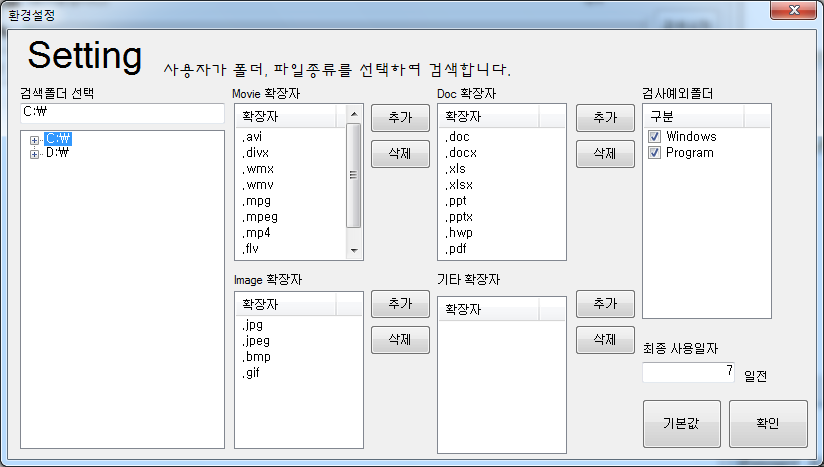
\includegraphics[width=0.7\textwidth]{Figures/Setting}
		\caption{환경설정}
		\label{fig:setting}
	\end{figure}
	\subsection{검색폴더 선택}
	모든 폴더 및 파일을 검색하는 것이 아닌 일부분의 폴더에서 검색을 하고 싶을때 사용한다. 하지만 다음 이미지와 같이 Program Files 나 Windows 폴더의 경우, 이후에 나올 검색예외폴더 설정창에서 체크박스를 해제하여야 검색이 가능하다.
	
	\begin{figure}[h]
		\centering
		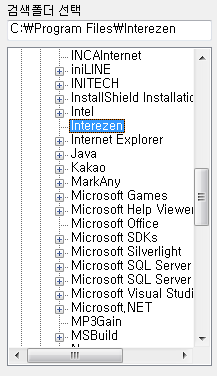
\includegraphics[height=0.35\textheight]{Figures/searchfolder}
		\caption{검색폴더 선택}
		\label{fig:searchfolder}
	\end{figure}
	
	\subsection{Movie 확장자}
	검색 파일 중 동영상 확장자를 가지고 있는 파일들을 메인 화면 내 동영상 섹션에 나열한다. 추가 버튼으로 동영상 섹션 내에서 검색하고 싶은 확장자를 더할 수 있으며 삭제 버튼으로 검색에서 제외하고 싶은 확장자를 제거 할 수 있다.
	
	\begin{figure}[h]
		\centering
		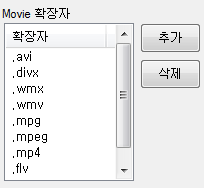
\includegraphics[width=0.4\textwidth]{Figures/Movie}
		\caption{Movie 확장자}
		\label{fig:movie}
	\end{figure}
	
\end{document}